\chapter{Sistema de Odometria Visual} \label{chap:sist}

Neste capitulo serão apresentados os procedimentos implementados para a realização dos testes. O capítulo aborda o \textit{software} e \textit{hardware} utilizados no desenvolvimento.

\section{Software}

Neste subcapítulo serão descritas as ferramentas de \textit{software} utilizadas bem como o código produzido.

\subsection{ROS}

ROS (\textit{Robot Operating System}) é uma \textit{framework} para desenvolvimento de \textit{sofware} de robótica. ROS consiste num compêndio de bibliotecas, ferramentas e outros recursos que visa facilitar a criação de comportamentos complexos alcançando uma vasta gama de plataformas robóticas distintas. 

O ROS fornece serviços idêntico a um sistema operativo, incluindo abstração de \textit{hardware}, baixo nivel de controlo, implementação de funcionalidades e mensagens que são transmitidas entre nós. Além disto , é constituido por bibliotecas e ferramentas para obter, criar, gravar e executar código em vários computadores. 

Desta forma, ROS  é caracterizado por :

\begin{itemize}
	\item \textbf{Pacotes} - O \textit{software} desenvolvido em ROS organiza-se em pacotes. Os pacotes são módulos que podem conter nós, bibliotecas independentes, \textit{datasets}, ficherisos de configuração, elementos de \textit{softwares} de terceiros, entre outros elementos que constituem o módulo. Os pacotes constituem a unidade base de compilação.
	\item \textbf{Nós} - Os nós são processos em ROS que executam computação, funcionando como programas. Os nós comunicam entre si através da publicação e subscrição de mensagens, serviços e através do \textit{Parameter Server}. Um sistema robótica em execução utiliza um conjunto de nós que cooperam para o seu funcionamento. A arquitectura distribuída de ROS permite que os nós em execução não necessitem de operar no mesmo equipamento, possibilitando a simbiose de diferentes plataformas comunicando entre si. O nó mestre pertence ao conjunto de nós laçando pelo \textit{roscore}, e tem a função de possibilitar aos nós que se localizem uns aos outros permitindo o estabelecimento de comunicações. 
	\item \textbf{Tópicos} - Os tópicos são os recipientes através dos quais os nós trocam mensagens  entre si. Os tópicos utilizam um modelo de publicação/subscrição que separa a produção de informação do seu consumo. Os nós não têm conhecimento de outros nós que publiquem determinado tópico ou o subscrevam. Um nó apenas necessita de subscrever os dados específicos a um tópico ou de publicar dados num tópico específico. A estrutura permite a existência de múltiplos publicadores e subscritores associados a cada tópico.
	\item \textbf{Serviços} - A unidirecionalidade existente no modelo publicador/subscritor não possibilita interações do tipo "pedido/resposta". Para possibilitar este tipo de interações existem os serviços em ROS. Um serviço é composto por um par de mensagens, uma mensagem definida para o pedido e outra para a resposta. Um nó pode oferecer um serviço ativado por um nó cliente ao submeter a mensagem de pedido.
 
\end{itemize}

A biblioteca de ROS suporta o desenvolvimento ROS em linguagem C++ e Python.

\subsubsection{Desenvolvimento em ROS}

Descrever os nós criados.

\subsection{Desenvolvimento em Matlab}

O Matlab é um \textit{software} de alto desempenho desenvolvido para o cálculo numérico. Caracteriza-se por implementar uma linguagem própria que resulta de uma combinação de linguagens como C, Java e Basic.

O código desenvolvido em Matlab teve como função principal o processamento dos dados guardados nos \textit{rosbags}. Estes \textit{rosbags} contêm as mensagens publicadas para cada teste realizado. Foram desenvolvidos \textit{scripts} para filtrar os dados de interesse e gerar dados possíveis de analisar e inferir conclusões.

\section{Hardware}

Este subcapítulo visa apresentar os componentes de hardware utilizado no desenvolvimento do projeto.

\subsection{Raspberry Pi}

O Raspberry Pi é um computador do tamanho de um cartão de crédito.Todo o hardware é integrado numa única placa. O principal objetivo é promover o ensino em Ciência da Computação básica em escolas mas, devido à sua excelente qualidade / preço é bastante usado em grandes projetos de robótica, programação e até aplicações industriais. 

O modelo utilizado nesta dissertação é o Raspberry Pi 3 model B. Es modelo contem um processador 1.2 GHz 64-bit quad-core ARMv8 CPU, 1 GB de RAM e Bluetooth 4.1. Além disto, este computador é compatível com ROS Kinetic e com vários módulos , quais como a câmara com lente olho de peixe.

\begin{figure}[h!] %colocar figura a seguir ao texto anterior
	\begin{center}
		\leavevmode		
		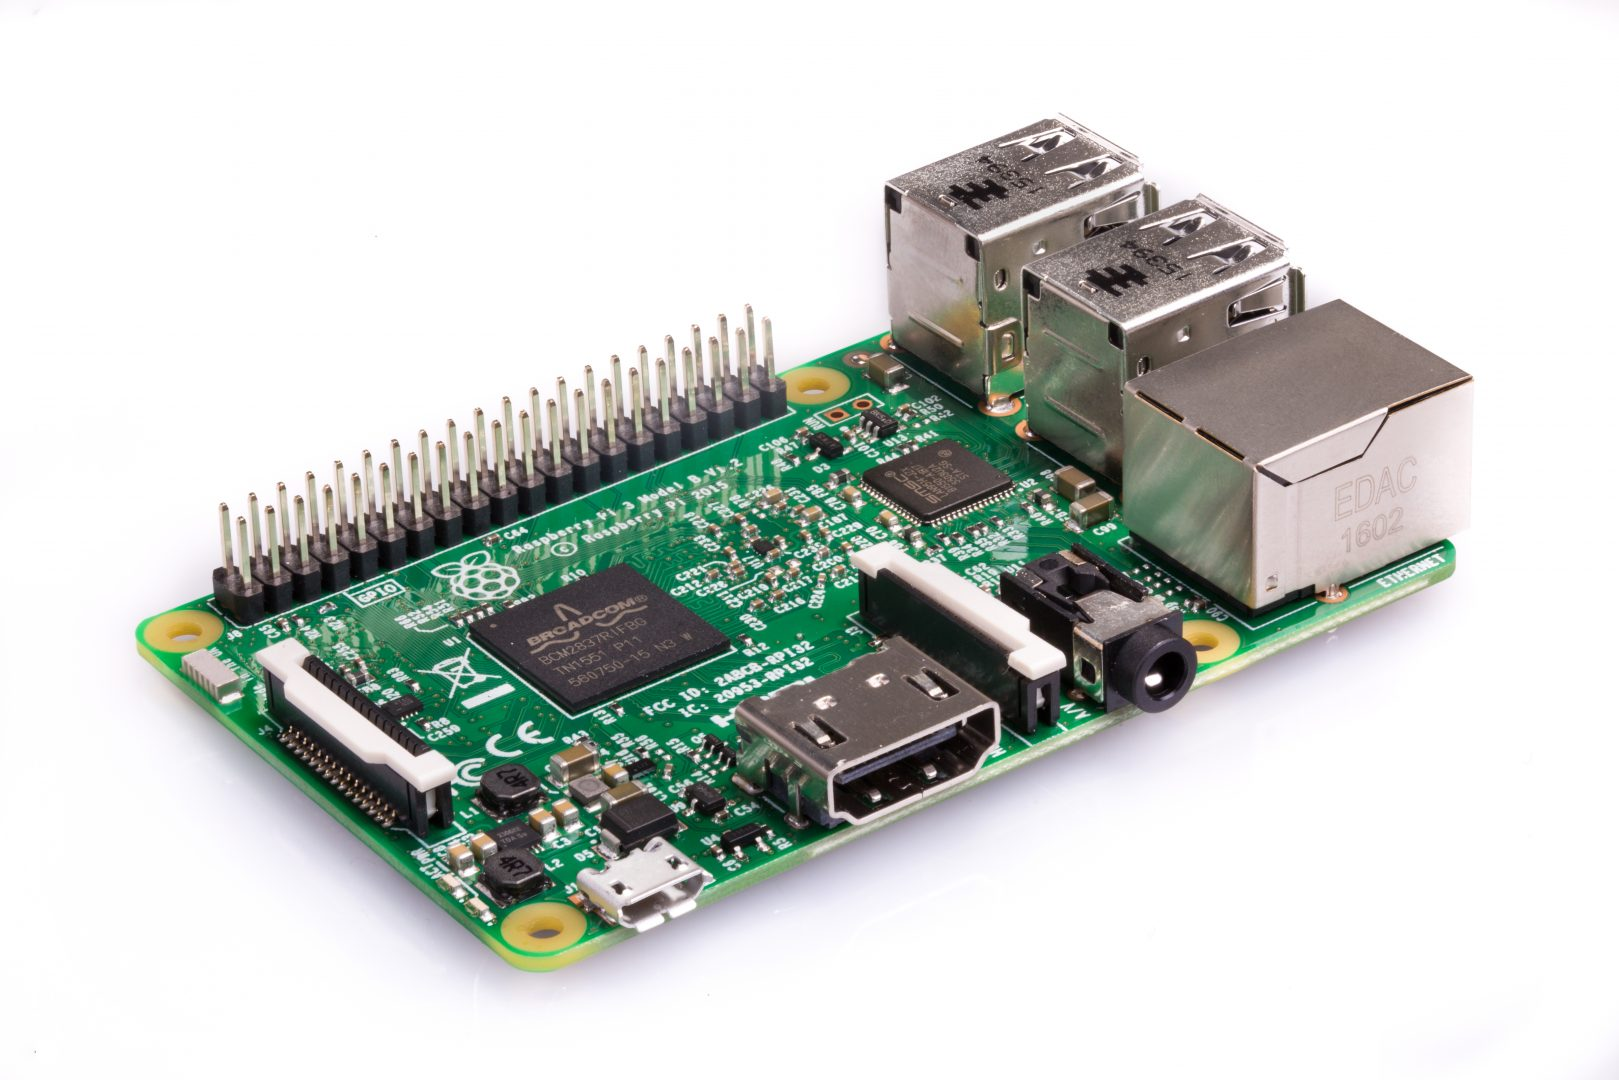
\includegraphics[width=0.6\textwidth]{raspberry.jpg}
		\caption{Exemplar da Raspberry Pi 3 modelo B.}
		\label{fig:raspberry}
	\end{center}
\end{figure}

\subsection{Câmara com lente olho de peixe}


\section{Configuração dos testes}

\subsection{Teste 1}

\subsection{Teste 2}
